\documentclass[12pt]{article}

\usepackage{amsmath}
\usepackage{amsfonts}
\usepackage{float}
\usepackage{fancyhdr}
\usepackage{graphicx}
\usepackage[colorlinks=true,linkcolor=blue, citecolor=red]{hyperref}
\usepackage{url}
\usepackage{parskip}
\usepackage[top=.75in, left=.5in, right=.5in, bottom=1in]{geometry}
\usepackage[utf8]{vietnam}
\setlength{\headheight}{29.43912pt}

% \graphicspath{PATH_TO_GRAPHIC_FOLDER}

\pagestyle{fancy}
\lhead{
\reportname
}
\rhead{
Trường Đại học Khoa học Tự nhiên - ĐHQG HCM\\
\coursename
}
\lfoot{\LaTeX\ by \href{https://github.com/trhgquan}{Quan, Tran Hoang}}

\newcommand{\coursename}{Mã hóa ứng dụng - CSC15003}
\newcommand{\reportname}{Trust Negotiation}
\newcommand{\trustx}{$\mathcal{\text{Trust-}X}$}

\begin{document}

\begin{titlepage}
\newcommand{\HRule}{\rule{\linewidth}{0.5mm}}
\centering

\textsc{\LARGE đại học quốc gia tphcm}\\[1.5cm]
\textsc{\Large trường đại học khoa học tự nhiên}\\[0.5cm]
\textsc{\large khoa công nghệ thông tin}\\[0.5cm]
\textsc{bộ môn công nghệ tri thức}\\[0.5cm]

\HRule \\[0.4cm]
{ 
\huge{\bfseries{Báo cáo Đồ án cuối kì}}\\[0.5cm]
\large{\bfseries{Đề tài: \reportname}}
}\\[0.4cm]
\HRule \\[0.5cm]

\textbf{\large Môn học: \coursename}\\[0.5cm]

\begin{minipage}[t]{0.4\textwidth}
\begin{flushleft} \large
\emph{Sinh viên thực hiện:}\\
Trần Hoàng Quân \textsc{(19120338)}\\
Lê Hoàng Trọng Tín \textsc{(19120682)}\\
Lê Mai Nguyên Thảo \textsc{(19120661)}
\end{flushleft}
\end{minipage}
~
\begin{minipage}[t]{0.4\textwidth}
\begin{flushright} \large
\emph{Giáo viên hướng dẫn:} \\
% Dr. James \textsc{Smith}
Thầy Trương Toàn Thịnh
\end{flushright}
\end{minipage}\\[2cm]

{\large \today}\\[2cm]


\includegraphics[scale=.25]{img/hcmus-logo.png}\\[1cm]

\vfill
\end{titlepage}
	
\tableofcontents
\pagebreak

\section{Trust Negotiation}
\subsection{Bài toán thực tế}
Xét qui trình thanh toán bằng thẻ tín dụng (hoặc thẻ NAPAS) ở siêu thị như sau:
\begin{enumerate}
\item Nhân viên thu ngân kiểm tra thẻ có hợp lệ hay không
\item Nhân viên thu ngân quẹt thẻ vào máy POS và cho khách hàng nhập mã PIN, số tiền.
\item Nhân viên thu ngân xác nhận thanh toán và in biên lai cho khách hàng ký.
\item Nhân viên thu ngân xác nhận chữ ký trên biên lai giống với chữ ký trên mặt sau của thẻ.
\end{enumerate}
Có thể nhận thấy, qui trình trên vẫn tiềm ẩn nhiều nguy cơ an ninh. Ví dụ, không phải ai cũng có kĩ năng chuyên môn để kiểm tra thẻ hợp lệ bằng mắt thường; không có gì đảm bảo nhân viên thu ngân không lợi dụng sơ hở của khách hàng để thay đổi số tiền, ..etc. Tuy tiềm ẩn nguy cơ, nhưng các giao dịch vẫn diễn ra hàng ngày vì sự tin tưởng của khách hàng với các tổ chức / nhãn hàng lớn.

Trên không gian số cũng vậy, phải có cách để tạo dựng sự tin cậy trong các giao dịch, các kết nối giữa các hệ thống với nhau. Đây cũng là lí do các giải pháp Trust Negotiation ra đời. Giống với thực tế, Trust Negotiation phải đạt được các mục tiêu sau:
\begin{itemize}
\item Tạo dựng sự tin cậy (Trust Establishment) giữa các bên tham gia.
\item Dù trao đổi các thông tin xác thực (credentials) với nhau, các thông tin này phải được giữ an toàn. 
\end{itemize}

\subsection{Trust Establishment (Thiết lập sự tin cậy)}
Mục tiêu của Trust Establishment là thiết lập sự tin cậy giữa những bên liên quan trong một hệ thống mở. Các bên này thường không cùng một miền bảo mật (security domain) với nhau, và do đó người ta thường không dùng danh tính (identity) mà dùng các thuộc tính (attributes) cho các thao tác xác thực sau này.

\subsection{Digital Credentials (Thông tin xác thực số)}
Digital Credentials chứa các thông tin dưới dạng thuôc tính của người / bên sở hữu và được cấp bởi một bên đáng tin cậy (thường là các ceritificate authority (CA) - nhà cung cấp chứng thư số).

Digital Credentials có các đặc điểm sau:
\begin{itemize}
\item Không thể làm giả.
\item Các thông tin được lưu trong Digital Credentials phải dễ xác thực.
\item Dùng PKI (public-key infrastructure, thường dùng chuẩn X.509 v3) để ký.
\end{itemize}

\subsection{Credential Disclosure Policy (CDP - Chính sách tiết lộ thông tin xác thực)}
Credential Disclosure Policy (CDP) là điều kiện đưa ra để một bên công bố các tài nguyên (resources) hoặc cho phép truy cập dịch vụ (services). Cần lưu ý là CDP áp dụng không chỉ cho resources và services. Vẫn có những policy áp dụng để bảo vệ credentials, kể cả CDP.

\subsection{Định nghĩa Trust Negotiation}
Trust Negotiation là phương pháp sử dụng cách tiếp cận kiểm soát truy cập (access control) và xác thực (authentication), cho phép bên yêu cầu tài nguyên (Resource Requester) và bên cung cấp tài nguyên (Provider) thiết lập sự tin cậy trên các hệ thống mở. Quá trình này dựa trên các thuộc tính (attributes) hơn là danh tính (identity).

Một số tính chất của Trust Negotiation:
\begin{itemize}
\item Trao đổi digital credentials môt cách tuần tự.
\item Mức độ nhạy cảm của credentials tăng dần khi độ tin cậy tăng dần.
\end{itemize}

\begin{figure}[H]
\centering
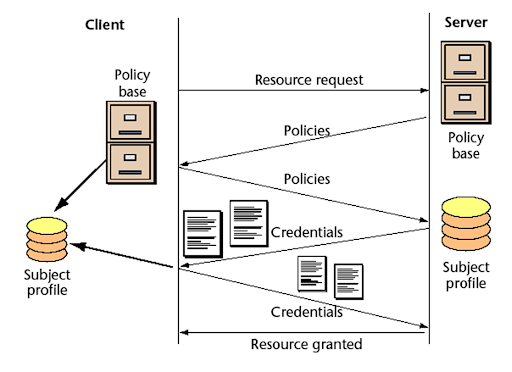
\includegraphics[scale=.5]{img/trust-simple.png}
\caption{Một mô hình Trust Negotiation đơn giản}
\label{fig:simple-trust}
\end{figure}

Các yêu cầu của một hệ thống Trust Management:
\begin{itemize}
\item Đảm bảo quyền sở hữu của credential.
\item Đảm bảo tính hợp lệ của credential.
\item Khám phá credential chain.
\item Có cơ chế bảo vệ quyền riêng tư.
\item Hỗ trợ các chiến thuật negotiate thay thế.
\begin{itemize}
\item Tăng cường bảo mật, tối ưu tính toán, ..etc
\end{itemize}
\item Các chiến thuật negotiate phải đảm bảo tốc độ (nhanh).
\end{itemize}

\section{Một số mô hình áp dụng Trust Negotiation}
Một số hệ thống Trust Management có thể kể đến:
\begin{itemize}
\item Keynote trust management system.
\item Trust Establishment phát triển bởi Haifa Research Lab.
\begin{itemize}
\item Trust Policy Language (TPL)\cite{848442}
\end{itemize}
\item TrustBuilder
\item Unipro
\item \trustx
\end{itemize}

Trong đó chúng ta đi sâu vào tìm hiểu các kiến trúc ATNAC và \trustx.

\subsection{ATNAC}
Adaptive Trust Negotiation and Access Control (ATNAC)\cite{10.1145/1063979.1064004}, là kiến trúc access control được ứng dụng vào các dịch vụ điện tử, sử dụng các hệ thống TrustBuilder và GAA-API.

\subsubsection{TrustBuilder}
Được phát triển bởi Đại học Brigham Young (BYU) và Đại học Illinois Urbana-Champaign (UIUC). Hệ thống chỉ thực hiên qui trình Trust Negotiation, tuy nhiên có nhiều khuyết điểm:
\begin{itemize}
\item Dễ bị tấn công DoS (denial of service - tấn công từ chối dịch vụ).
\begin{itemize}
\item Attacker gửi số lượng lớn sessions lên server khiến hệ thống bị nghẽn.
\item Các policy có chi phí tính toán phức tạp, tốn nhiều thời gian tính toán.
\item Tính toán và xác thực các credentials không hợp lệ hoặc không liên quan gây lãng phí. 
\end{itemize}
\item Các cuộc tấn công vào hê thống TrustBuilder thường nhắm vào các thông tin nhạy cảm.
\end{itemize}
Để khắc phục khuyết điểm này, ATNAC sử dụng middleware GAA-API.

\subsubsection{GAA-API}


\subsection{\trustx}
\trustx\cite{10.1109/TKDE.2004.1318565} là một kiến trúc thiết kế riêng cho kiểu tương tác P2P (Peer-to-Peer)

\addcontentsline{toc}{section}{Tài liệu}
\bibliographystyle{plain}
\bibliography{sample}

\end{document}